\documentclass[11pt]{article}

% ---------- Page & fonts ----------
\usepackage[margin=1in]{geometry}
\usepackage[utf8]{inputenc}
\usepackage[T1]{fontenc}
\usepackage{xcolor}

% ---------- Math ----------
\usepackage{amsmath, amssymb, amsthm, mathtools}

% ---------- Graphs / figures ----------
\usepackage{tikz}
\usetikzlibrary{positioning, arrows.meta, calc}

% ---------- Quality of life ----------
\usepackage{enumitem}
\usepackage{hyperref}
\usepackage{cleveref}
\usepackage{xcolor}

\hypersetup{
  colorlinks=true,
  linkcolor=blue!50!black,
  citecolor=blue!50!black,
  urlcolor=blue!50!black
}

% ================= Theorem environments =================
\theoremstyle{plain}
\newtheorem{theorem}{Theorem}[section]
\newtheorem{lemma}[theorem]{Lemma}
\newtheorem{proposition}[theorem]{Proposition}
\newtheorem{corollary}[theorem]{Corollary}
\newtheorem{conjecture}[theorem]{Conjecture}

\theoremstyle{definition}
\newtheorem{definition}[theorem]{Definition}
\newtheorem{example}[theorem]{Example}
\newtheorem{exercise}[theorem]{Exercise}

\theoremstyle{remark}
\newtheorem{remark}[theorem]{Remark}
\newtheorem*{note}{Note}

% ================= Graph theory macros =================
% Sets
\newcommand{\V}{V}                       % vertex set
\newcommand{\E}{E}                       % edge set
\newcommand{\N}{N}                       % neighbourhood, N(v)

% Common graph families
\newcommand{\Kn}[1]{K_{#1}}              % complete graph K_n
\newcommand{\Kmn}[2]{K_{#1,#2}}          % complete bipartite K_{m,n}
\newcommand{\Cn}[1]{C_{#1}}              % cycle
\newcommand{\Pn}[1]{P_{#1}}              % path

% Invariants (as operators, upright text, correct spacing)
\DeclareMathOperator{\dg}{d}             % degree, use dg(v) to avoid clashing with \deg
\DeclareMathOperator{\ex}{ex}            % extremal function ex(n, H)
\DeclareMathOperator{\girth}{girth}
\DeclareMathOperator{\diam}{diam}
\DeclareMathOperator{\Aut}{Aut}
\DeclareMathOperator{\chr}{\chi}          % chromatic number, use \chr(G)
\DeclareMathOperator{\comp}{c}            % number of components

% Misc shorthands
\newcommand{\iso}{\cong}                 % isomorphic
\newcommand{\subgraph}{\subseteq}        % spanning/sub relations, adjust as needed

% ================= TikZ Styles =================
\tikzset{
    vertex/.style={
        circle,
        draw=black,
        fill=black,
        inner sep=1.8pt
    },
    edge/.style={
        thick
    },
    rededge/.style={
        thick,
        red
    },
    blueedge/.style={
        thick,
        blue
    }
}

% ================= Document =================
\title{Linear Arboricity}
\author{Siddharth Narayan Mishra}
\date{\today}

\begin{document}

\maketitle

The \textbf{linear arboricity} of a graph $G$, denoted by $la(G)$, is the minimum number of linear forests into which the edge set $E(G)$ can be partitioned.

Equivalently, we seek to colour every edge of $G$ using as few colours as possible so that every colour class induces a linear forest.

\paragraph{Intuition}

A linear forest is simply a collection of disjoint paths. Therefore, the linear arboricity asks the following question:

\begin{quote}
How many collections of paths are needed so that every edge of the graph belongs to exactly one collection?
\end{quote}

The smaller this number, the "closer" the graph is to already being a collection of paths.

\paragraph{Example 1: A Path}

Consider the path $P_4$.

\begin{center}
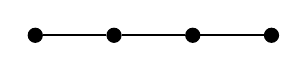
\begin{tikzpicture}
\node[vertex] (a) at (0,0) {};
\node[vertex] (b) at (1,0) {};
\node[vertex] (c) at (2,0) {};
\node[vertex] (d) at (3,0) {};

\draw[edge] (a)--(b)--(c)--(d);
\end{tikzpicture}
\end{center}

The graph itself is already a linear forest since it consists of exactly one path.

Hence,

\[
la(P_4)=1.
\]

\paragraph{Example 2: A Triangle}

Consider the cycle $C_3$.

\begin{center}
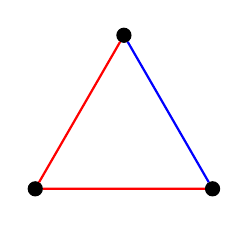
\begin{tikzpicture}

\node[vertex] (A) at (90:1.3) {};
\node[vertex] (B) at (210:1.3) {};
\node[vertex] (C) at (330:1.3) {};

\draw[rededge] (A)--(B)--(C);
\draw[blueedge] (C)--(A);

\end{tikzpicture}
\end{center}

The red edges form one path, while the blue edge forms another path.

Each colour therefore represents one linear forest.

Hence,

\[
la(C_3)=2.
\]

\paragraph{Example 3: A Star}

Consider the star graph $K_{1,3}$.

\begin{center}
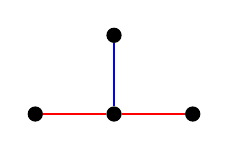
\begin{tikzpicture}

\node[vertex] (O) at (0,0) {};
\node[vertex] (A) at (-1,0) {};
\node[vertex] (B) at (1,0) {};
\node[vertex] (C) at (0,1) {};

\draw[rededge] (A)--(O);
\draw[rededge] (O)--(B);
\draw[blueedge] (O)--(C);

\end{tikzpicture}
\end{center}

Although $K_{1,3}$ is a tree, it is not a linear forest because the centre vertex has degree $3$.

The red edges form one path and the blue edge forms another.

Therefore,

\[
la(K_{1,3})=2.
\]

\paragraph{Remark}

Notice that the graph itself does \emph{not} have to be a linear forest. We only require that its edges can be partitioned into linear forests.

%=========================================================
\hrulefill
\section*{Linear Forest}

A \textbf{linear forest} is a forest in which every connected component is a path.

Equivalently, a graph is a linear forest if and only if

\begin{itemize}
    \item it contains no cycles, and
    \item every vertex has degree at most $2$.
\end{itemize}

The first condition prevents cycles, while the second prevents branching.

\paragraph{Examples}

The following are linear forests.

\begin{center}
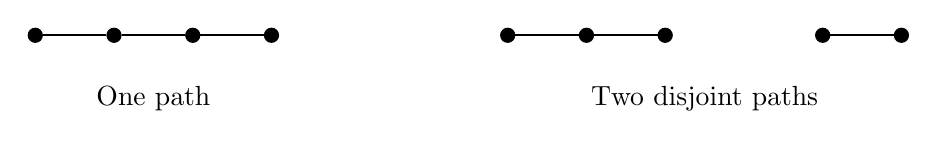
\begin{tikzpicture}[scale=1]

%---------------- First Example ----------------

\node[vertex] (a1) at (0,0) {};
\node[vertex] (a2) at (1,0) {};
\node[vertex] (a3) at (2,0) {};
\node[vertex] (a4) at (3,0) {};

\draw[edge] (a1)--(a2)--(a3)--(a4);

\node at (1.5,-0.8) {One path};

%---------------- Second Example ----------------

\node[vertex] (b1) at (6,0) {};
\node[vertex] (b2) at (7,0) {};
\node[vertex] (b3) at (8,0) {};

\node[vertex] (b4) at (10,0) {};
\node[vertex] (b5) at (11,0) {};

\draw[edge] (b1)--(b2)--(b3);
\draw[edge] (b4)--(b5);

\node at (8.5,-0.8) {Two disjoint paths};

\end{tikzpicture}
\end{center}

Both graphs consist entirely of paths.

Hence both are linear forests.

\paragraph{Non-examples}

\begin{center}
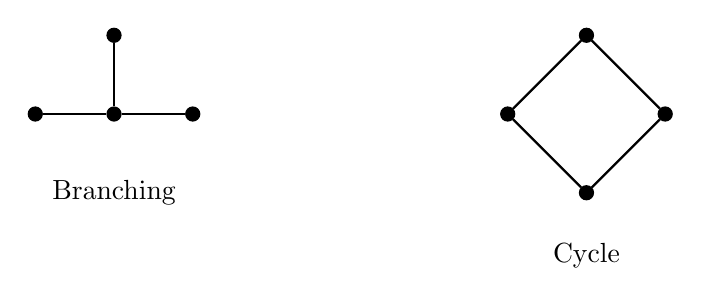
\begin{tikzpicture}

%---------------- Branching ----------------

\node[vertex] (c) at (0,0) {};
\node[vertex] (l) at (-1,0) {};
\node[vertex] (r) at (1,0) {};
\node[vertex] (u) at (0,1) {};

\draw[edge] (l)--(c)--(r);
\draw[edge] (c)--(u);

\node at (0,-1.0) {Branching};

%---------------- Cycle ----------------

\node[vertex] (d1) at (5,0) {};
\node[vertex] (d2) at (6,1) {};
\node[vertex] (d3) at (7,0) {};
\node[vertex] (d4) at (6,-1) {};

\draw[edge] (d1)--(d2)--(d3)--(d4)--(d1);

\node at (6,-1.8) {Cycle};

\end{tikzpicture}
\end{center}

The graph on the left is a tree but not a path because one vertex has degree $3$.

The graph on the right contains a cycle.

Therefore, neither graph is a linear forest.

\paragraph{Remarks}

\begin{itemize}
    \item Every path is a linear forest.
    \item Every linear forest is a forest.
    \item Every connected linear forest is a path.
    \item Every vertex of a linear forest has degree at most $2$.
\end{itemize}

%=========================================================
\hrule
\subsection*{Forest}

A \textbf{forest} is a graph that contains no cycles.

Equivalently, every connected component of a forest is a tree.

\paragraph{Examples}

\begin{center}
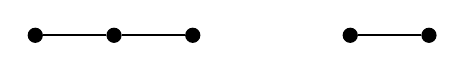
\begin{tikzpicture}

% Tree 1
\node[vertex] (a) at (0,0) {};
\node[vertex] (b) at (1,0) {};
\node[vertex] (c) at (2,0) {};

\draw[edge] (a)--(b)--(c);

% Tree 2
\node[vertex] (d) at (4,0) {};
\node[vertex] (e) at (5,0) {};

\draw[edge] (d)--(e);

\end{tikzpicture}
\end{center}

This graph is a forest consisting of two trees.

A connected forest is simply called a tree.

\paragraph{Non-example}

\begin{center}
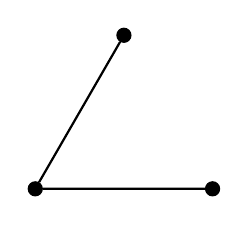
\begin{tikzpicture}

\node[vertex] (A) at (90:1.3) {};
\node[vertex] (B) at (210:1.3) {};
\node[vertex] (C) at (330:1.3) {};

\draw[edge] (A)--(B)--(C)--cycle;

\end{tikzpicture}
\end{center}

This graph is not a forest because it contains a cycle.

\paragraph{Remarks}

\begin{itemize}
    \item Every tree is a forest.
    \item A forest may be connected or disconnected.
    \item A forest with exactly one connected component is a tree.
\end{itemize}

\[
\boxed{\text{Tree}\subseteq\text{Forest}.}
\]


\end{document}